\documentclass[11pt]{article}

% ------
% LAYOUT
% ------
\textwidth 165mm %
\textheight 230mm %
\oddsidemargin 0mm %
\evensidemargin 0mm %
\topmargin -15mm %
\parindent= 10mm

\usepackage[dvips]{graphicx}
\usepackage{multirow,multicol}
\usepackage[table]{xcolor}

\usepackage{amssymb}
\usepackage{amsfonts}
\usepackage{amsthm}
\usepackage{amsmath}

\usepackage{subfigure}
\usepackage{minted}

\graphicspath{{./pix/}} % put all your figures here.

\begin{document}
\begin{center}
\Large{\textbf{ECE 595: Homework 6}}

Yi Qiao, Class ID 187

(Spring 2019)
\end{center}

\section*{Exercise 1: Hoeffding Inequality}
\subsection*{(a) probability of getting a head for coins $c_1$, $c_{rand}$ and $c_{min}$}
Since they are all fair coins,
$$\mathbb{P}(c_1=head)=\mathbb{P}(c_{rand}=head)=\mathbb{P}(c_{min}=head)=0.5$$
\subsection*{(b) python experiment}
\begin{figure}[h]
	\centering
	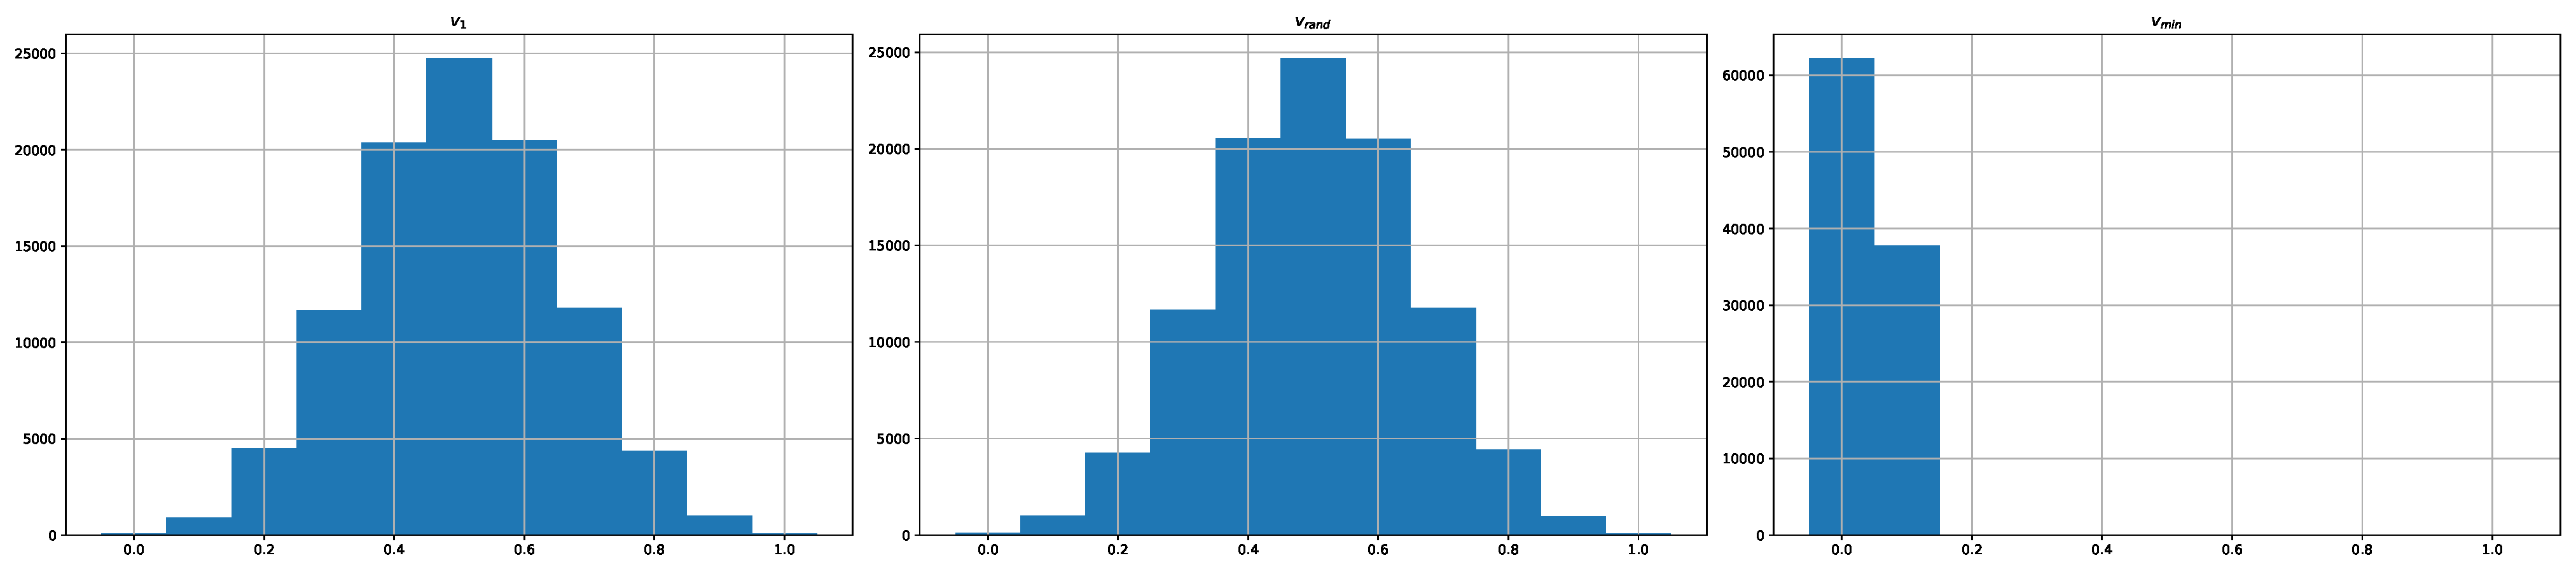
\includegraphics[width=\linewidth]{exercise1_b}
\end{figure}
\subsection*{(c) plots}
\begin{figure}[h]
	\centering
	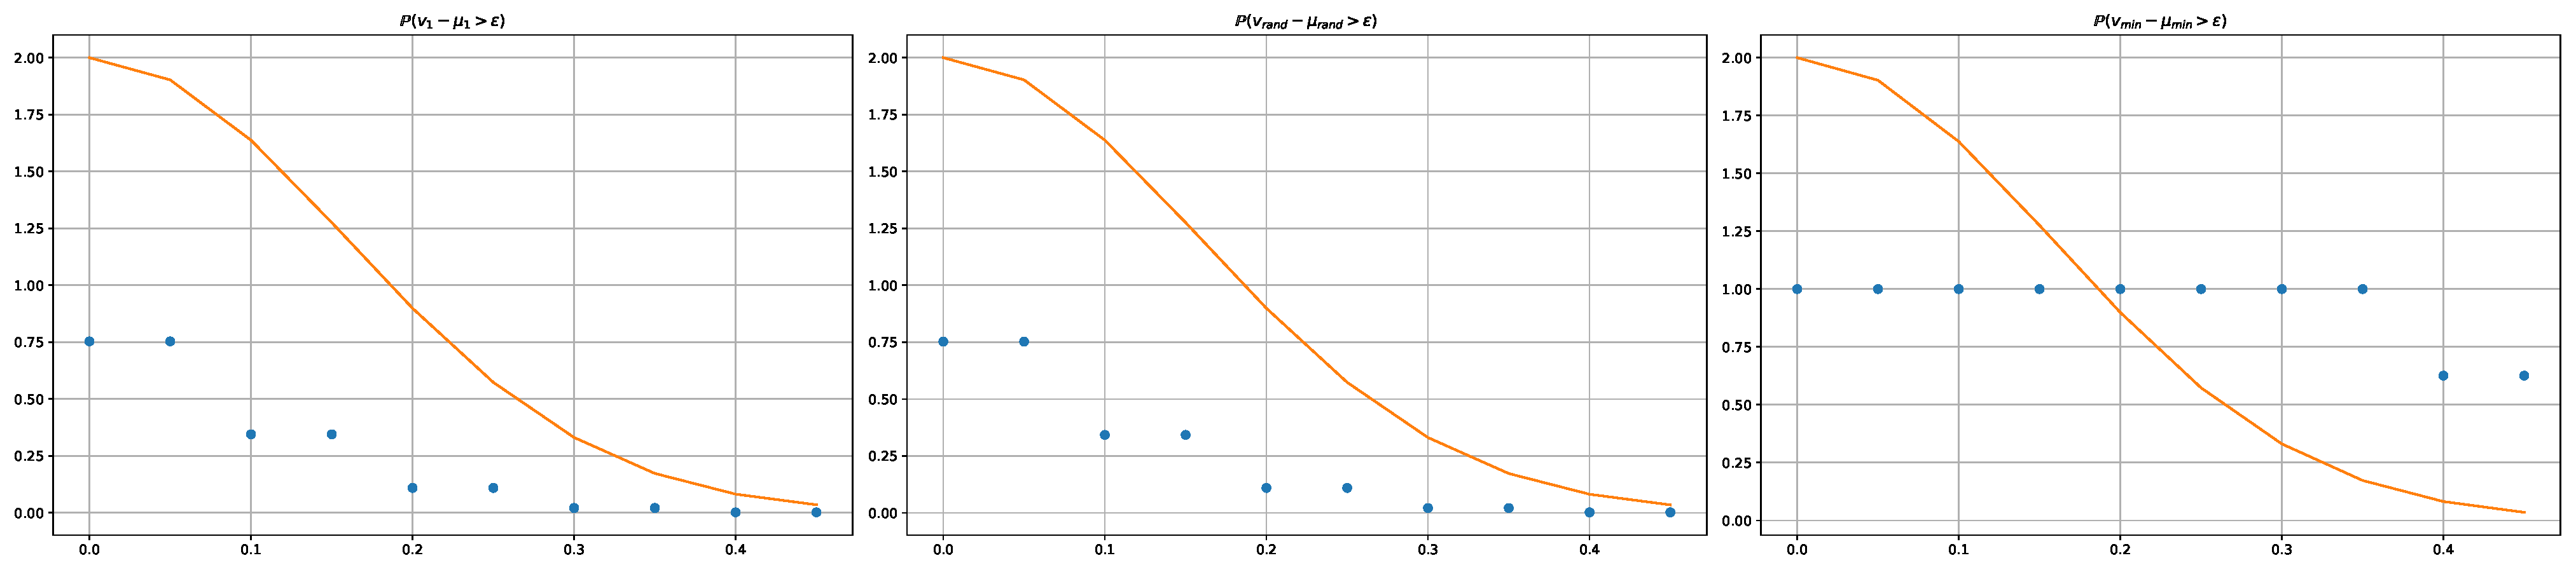
\includegraphics[width=\linewidth]{exercise1_c}
\end{figure}
\subsection*{(d)}
By observation, we can see that the first two obviously obey the Hoeffding's bound while the third one does not.
\subsection*{(e)}
something something...
\pagebreak
\section*{Exercise 2: VC Dimension}
\subsection*{(a) Compute the VC dimension}
\subsubsection*{(i)}
\begin{equation}
\begin{split}
\mathcal{H}=&\{h:\mathbb{R}\rightarrow\{-1,+1\}|h(x)=+1,\forall x\in[a,\infty), a\in\mathbb{R}\} \cup \\
&\{h:\mathbb{R}\rightarrow\{-1,+1\}|h(x)=+1,\forall x\in(-\infty,a], a\in\mathbb{R}\}
\end{split}
\end{equation}
By inspection, the VC dimension of the above hypothesis set is 2.

\subsubsection*{(ii)}
\begin{equation}
\begin{split}
\mathcal{H}=&\{h:\mathbb{R}\rightarrow\{-1,+1\}|h(x)=+1,\forall x\in[a,b], a,b\in\mathbb{R}\} \cup \\
&\{h:\mathbb{R}\rightarrow\{-1,+1\}|h(x)=-1,\forall x\in[a,b], a,b\in\mathbb{R}\}
\end{split}
\end{equation}
By inspection, the VC dimension of the above hypothesis set is 3.

\subsubsection*{(iii)}
\begin{equation}
\begin{split}
\mathcal{H}=&\left\{h:\mathbb{R}^d\rightarrow\{-1,+1\}|h(x)=+1,\forall x\ where \sqrt{\sum_{j=1}^{d} x_j^2}\le b, b\in\mathbb{R}\right\}
\end{split}
\end{equation}

By inspection, hypothesis function is a hyper ball. Thus, the VC dimension of the above hypothesis set is 1.

\subsection*{(b)}
\begin{equation}
\begin{split}
\mathcal{H}=&\left\{h_\alpha:\mathbb{R}\rightarrow\mathbb{R}|h_\alpha(x)=(-1)^{\lfloor \alpha x\rfloor},\alpha\in\mathbb{R}\right\}
\end{split}
\end{equation}
Even though the above hypothesis set has only one parameter, it is periodic, thus by tuning the period/frequency, you can match any number of data points you want by finding their GCD.
This hypothesis set has simply too large VC dimension, which is far beyond the model complexity. Thus, this will perform far worse than perceptron due to over-fitting.

\pagebreak
\section*{Exercise 3: Bias-Variance Trade-off}
\end{document}


